\documentclass{article}

\usepackage{caption}
\usepackage{amsmath}
\usepackage{amssymb}
\usepackage{graphicx}
\usepackage{tikz}
\usetikzlibrary{shapes.geometric}
\usetikzlibrary{arrows.meta}

\title{Volumes of Revolution and Differential Equations (Assessment)}
\author{Zac Hart}

\graphicspath{{./images/}}

\DeclareCaptionLabelFormat{custom}{Fig. #2}
\captionsetup{format=hang, labelformat=custom, labelsep=period, labelfont=bf}

\begin{document}

\begin{titlepage}
    \maketitle
    \tableofcontents
\end{titlepage}

\section{Answers}

\subsection{Cylindrical Shells and Washers}

There are two methods for finding the volume of a solid of revolution.
\begin{enumerate}
    \item The cylindrical shell method involves dividing the solid of revolution into cylindrical shells. By integrating the volumes of all of these shells, the total volume of the solid can be found.

    \begin{figure}[h]
        \label{fig:1}
        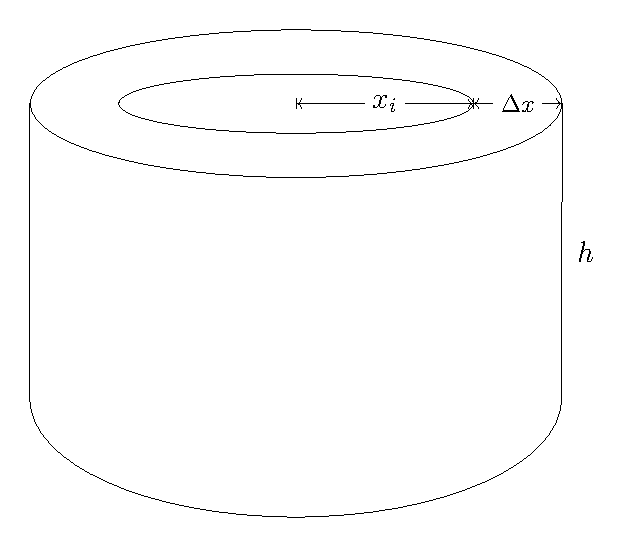
\includegraphics[width=\textwidth]{figure-1.pdf}
        \caption{A cylindrical shell.}
    \end{figure}
\end{enumerate}

\end{document}
